\newpage
\section{Vorbereitungsfragen}
\subsection{Photovoltaik-Inselanlage}
\subsubsection{Anlagenkonzepte von PV-Inselanlagen }
<<<<<<< HEAD
Anlagenkonzepte unterscheiden sich durch die verwendeten
Komponenten, die Verschaltung und die angeschlossenen Verbraucher.\\
Das einfachste Konzept ist das direkte Verschalten der PV-Anlage mit
=======
Die Konzepte unterscheiden sich durch die verwendeten
Komponenten, die Verschaltung und die angeschlossenen Verbraucher.\\
Das Einfachste der vier Konzepte ist das direkte Verschalten der PV-Anlage mit
>>>>>>> 54e1827e4e21b7f7edc93a2134db3186f16d27ea
DC-Verbrauchern, hierbei kann es sich z.B. um ein Heizungssystem für ein Schwimmbecken handeln.\\
Das zweite System wird durch eine Batterie ergänzt welche zwischen die PV-Anlage und die Verbraucher geschaltet ist.
Mögliche Anwendungen sind einfache DC-Systeme, welche allerdings auch außerhalb der Sonnenstunden
funktionieren müssen und dementsprechend einen Puffer benötigen. Ein Beispiel wäre hier ein solarversorgter Snackautomat.\\
Das komplexeste System, welches weiterhin für DC-Verbraucher gedacht ist, wird neben den Komponenten des zweiten Systems
um einen Laderegler ergänzt welcher vor die Batterie geschaltet wird. Solche Systeme werden häufig in
Wohnmobilen oder Wohnwägen verwendet, welche mit DC-Verbrauchern ausgestattet sind.\\
Um AC-Verbraucher nutzen zu können muss System 3 um einen Umrichter erweitert werden, welcher vor die Verbraucher geschaltet wird. Diese Systeme können dann Einfamilienhäuser, Forschungsstationen oder abgelegene Dörfer versorgen und ein Netz etablieren.\\ 
<<<<<<< HEAD
\subsubsection{Prüfung der Funktionsfähigkeit von Anlagenkomponenten}
Gemessen werden an allen Ein- und Ausgängen der Geräte sowohl der Strom als auch die Spannung.
=======
\subsubsection{Die Anlagenkomponenten sollen im Inselsystem auf ihre Funktionsfähigkeit hin geprüft werden. Was messen sie in welcher Reihenfolge?}
Gemessen wird an allen Ein- und Ausgängen der Geräte sowohl der Strom als auch die Spannung.
>>>>>>> 54e1827e4e21b7f7edc93a2134db3186f16d27ea
Beginnend mit dem Ausgang der PV-Anlage, wird dann entlang der Erzeugungslinie geprüft.
So folgt die Prüfung des Ladereglers. Anschließend wird das Batteriesystem geprüft und abschließend der Umrichter.\\


\subsection{Laderregler}
\subsubsection{Voraussetzungen für Anlagen mit Akku ohne Laderegler}
Inselnetzanlagen müssen in der Lage sein, die Ladung des Akkus und die Stromversorgung des angeschlossenen Verbrauchers zu gewährleisten. Dementsprechend müssen die einzelnen Bauteile aufeinander ausgelegt werden, um eine Beschädigung der Komponenten zu vermeiden. Ein Laderegler wird benötigt, sobald die Leerlaufspannung der Module die maximale Ladespannung der Batterie überschreitet, eine spannungsunabhängige Schaltung umgesetzt werden soll (bei größeren Anlagen) oder keine konstanten Wetterbedingungen garantiert werden können. Ein Laderegler sorgt dafür die Batterie vor Tiefenentladung und/oder Überladung zu schützen. In Kombination mit einem MPP-Tracker kann ein Laderegler auch den Energieertrag erhöhen. 
\subsubsection{Verfahren zur Laderegelung}
Es wird in drei unterschiedliche Arten von Ladereglern (LR) unterschieden:
\begin{itemize}
\begin{figure}[!h]
		\centering
		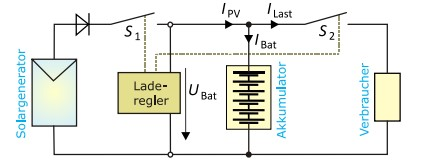
\includegraphics[width=0.7\textwidth]{Abbildungen/Serienladeregler}
		\caption{Photovoltaik-Batteriesystem mit einem Serienladeregler  }
		\label{fig:Serienladeregler}
\end{figure}
\item In Serienladereglern (auch Längsregler) (\autoref{fig:Serienladeregler}) werden Leistungshalbleiter als Schalter verwendet um den Stromfluss zu unterbrechen. Das hat zur Folge, dass beim Laden des Akkus immer Durchlassverluste entstehen. Serienladeregler sind die preiswertesten LR und können auch für nicht kurzschlussfeste Verbraucher genutzt werden. 

\begin{figure}[!h]
		\centering
		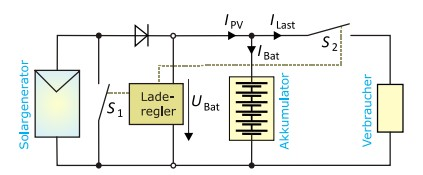
\includegraphics[width=0.7\textwidth]{Abbildungen/Shuntladeregler}
		\caption{Photovoltaik-Batteriesystem mit einem Shuntladeregler}
		\label{fig:Shuntladeregler}
\end{figure}

\item Shuntregler (auch Parallelregler) (\autoref{fig:Shuntladeregler}) sind am weitesten verbreitet. Diese schalten bei vollgeladenem Akku den Solargenerator kurz. Dieser Kurzschluss stellt im regulären Betrieb kein Problem dar, kann aber bei Abschattungen zu extremen Belastungen einzelner Zellen führen.

\item MPP-Laderegler können auch bei wechselnden Wetterbedingungen beste Ladeleistungen erreichen. Nachteilig sind allerdings die hohen Anschaffungskosten.

\end{itemize}
\subsubsection{Austausch defekter Batterien}
Das Wechseln der Batterie erfolgt in sieben einzelnen Schritten. Als erstes sollte die Betriebsanleitung gelesen und danach die Last abgeschaltet und vom System getrennt werden. Darauffolgend muss sowohl der PV-Generator als auch die Batterie vom Laderegler getrennt werden. Nun kann die neue Batterie und dann der PV-Generator an den Laderegler angeschlossen werden. Als letztes wird die Last wieder angeschaltet.
\newpage
\subsection{Batteriesysteme}
\subsubsection{Vor- und Nachteile von 2 Batterietypen}
Die beiden am häufigsten verwendeten Akkumulatoren sind Blei- und Lithium-Ionen-Akkus.
Blei Akkus haben zum Vorteil, dass sie schon sehr lange, beispielsweise für Kraftfahrzeuge, in der Benutzung sind und so sehr weit optimiert werden konnten. Außerdem sind die Speicher preiswert und leicht zu erwerben. Nachteilig sind sowohl die geringe Energiedichte (im Vergleich mit Lithium Akkus) als auch die Selbstentladung von ca. 10\% pro Monat (bei 25°C). Um eine Tiefenentladung zu vermeiden, müssen Bleiakkumulatoren deshalb regelmäßig nachgeladen werden. Dazukommend darf der Akku nicht mit zu hoher Spannung geladen werden um Gasungen und Wasserverluste zu vermeiden. Deshalb muss bei der Wahl eines Batterieraums auf eine gute Durchlüftung geachtet werden.\\\\
Lithium-Ionen-Akkus zeichnen sich durch ihre hohe Energiedichte und geringe Selbstentladerate aus. Beachtet werden muss allerdings der höhere Preis und die zeitweilig geringe Verfügbarkeit auf Grund der hohen Nachfrage. Ein weiterer Nachteil ist die Empfindlichkeit der Batteriezellen, weshalb diese mit einem elektronischem Batteriemanagementsystem überwacht und geschützt werden müssen.\\\\
Bei der Ladereglung von Batteriesystemen ist es besonders wichtig auf die Ladeströme und Spannungen, die Batterieräume als auch auf die Empfindlichkeit der Batteriezellen zu achten, um Beschädigungen des Systems zu vermeiden.

\subsubsection{ Anforderungen an Batterieräume }
Ein Batterieraum sollte trocken, gut belüftet, mit einem Rauchmelder ausgestattet und gleichmäßig im zulässigen Temperaturbereich temperiert sein.
\subsubsection{Häufig eingesetzten Systemspannungen}
Häufige eingesetzte Systemspannungen sind 12 V, 24V, 48V, und 72V.
Bei DC-Verbrauchern kann es zu hohen Strömen kommen, weshalb große Kabelquerschnitte vorteilhafter sind.
\newpage
\subsection{Wechselrichter in PV-Inselanlagen}
\subsubsection{Auswahlkriterien eines Insel-Wechselrichters}
\begin{itemize}
    \item Die Leistung des Umrichters muss an die Leistungsanforderungen des Insel-Netzes angepasst werden.
    \item Die Signalqualität der Spannung muss auch unter Last in den erforderten Grenzen der Verbraucher bleiben.
    \item Der Wirkungsgradbereich muss nach dem Lastverhalten des Inselnetzes ausgelegt werden.
    \item Der Umrichter muss die gleiche Phasen-Anzahl besitzen wie das System benötigt.
\end{itemize}
\subsubsection{Insel-Wechselrichter-Typen}
Mögliche Umrichter Typen:
\begin{itemize}
    \item mit oder ohne inneren Trafo
    \item 3 Level oder Multi Level
    \item ein oder drei Phasig
    \item Single- oder Multistring
\end{itemize} 
\subsubsection{Schlechte Wechselrichter}

\begin{itemize}
    \item Die Qualität der Spannung ist durch Oberschwingungen und Verzerrungen unzureichend.
    \item Der Umrichter produziert zu große Mengen an Wärme im Nennlast betrieb.
    \item Der Momentan-Wirkungsgrad des Wechselrichters kann mit Hilfe von \autoref{eq:230430_WR-Wirkungsgrad} bestimmt werden.
    \item Wenn der Wirkungsgrad bei Nennleistung deutlich unter einem wert von 90\% liegt, kann der Umrichter als 'schlecht' bezeichnet werden.
\end{itemize}

\begin{equation}
    \eta_{WR} = \frac{P_{WR,Ein}}{P_{WR,Aus}}
    \label{eq:230430_WR-Wirkungsgrad}
\end{equation}

\subsubsection{Anforderungen an den Einbauort eines Wechselrichters}
\begin{itemize}
    \item Der Einbauort muss vor Witterung schützen.
    \item Der Umrichter muss gut belüftet sein.
    \item Die Umgebungstemperatur des Umrichters, darf zu keiner zeit außerhalb seines angegebenen Temperaturbereichs liegen.
    \item Die Umrichter sollten für Wartungszwecke leicht zugänglich sein.
    \item Ein Brand sollte möglichst schnell erkannt werden, durch z.B. Brandmelder und sollte keine anderen Komponenten beeinflussen (durch genügend Abstand oder Abschirmung).
\end{itemize}
\subsubsection{Sofortige Lastabschaltung des Wechselrichters}
Bei jedweder Gefahr für die Verbraucher:
\begin{itemize}
    \item Überspannungen durch z.B. Blitzeinschlag
    \item Kurzschlüsse durch z.B. Hochwasser
    \item Feuer am Umrichter.
\end{itemize}
\subsubsection{Auswirkungen der benötigten Blindleistung auf Dimensionierung des Wechselrichters}
Durch zusätzlich benötigte Blindleistung muss der Umrichter nicht auf die Leistung des PV-Generators ausgelegt werden, sondern auf die Scheinleistung, welches er ins Netz geben muss.
Diese wird also zusätzlich innerhalb des Umrichters generiert, führt aber zu größeren Leistungflüssen.\cite{SMA_Q-Auslegung}
\subsubsection{Ein PC (einschließlich Peripherie) benötigt 120 W. Der Inselwechselrichter der unter 3. beschriebenen Anlage schaltet wegen Batterieerschöpfung nach 2 Tagen Betriebsdauer ab. Welche Möglichkeit des Dauerbetriebs der Anlage schlagen Sie vor. Begründen Sie die Realisierbarkeit.}
Es wird ein sowohl Spannung als auch Strom regelnder Umrichter benötigt, um zwischen Insel- und Netzbetrieb wechseln zu können.
\newpage
\subsection{Einstrahlung und Umgebungsbedingungen}
\subsubsection{Messverfahren zur Erfassung der Globalstrahlung}
Es gibt 2 Physikalische Effekte, welche konventionell zur Messung der Globalstrahlung verwendet werden. 
Der Photo-Effekt, welcher in Pyranometern mit Halbleitersensoren verwendet wird. 
Dieser Basiert auf dem selben Prinzip wie eine Photovoltaikzelle und setzt die Einstrahlung in Proportion mit dem Strom.
Der Seebeck-Effekt wird genutzt, welcher in thermischen Pyranometern zur Anwendung kommt.
Es wird eine von zwei miteinander verbundenen Metallplatten durch die Bestrahlung aufgeheizt. 
Der Seebeck-Effekt besagt, dass durch eine Temperaturdifferenz zwischen 2 Leitermaterialien eine elektrische Spannung entsteht.\cite{Wiki-Seebeck}
Dies hat den Vorteil, dass ein viel größerer Teil des Spektrums gemessen wird.

\subsubsection{Einfluss diffuser und direkter Sonnenstrahlung auf die Leistung des PV-Generators}
Der PV-Generator kann problemlos sowohl bei direkter als auch diffuser Bestrahlung Leistung entnehmen. 
Jedoch hat die diffuse Einstrahlung eine geringere spezifische Leistung, da sie mehr Weg durch die Atmosphäre zurückgelegt hat und somit einige Wellenlängen durch Absorptionsbänder herausgefiltert wurden.
\subsubsection{Modultemperatur}
Die Modultemperatur wird durch mehrere Faktoren beeinflusst: die Umgebungstemperatur, die Bestrahlungsstärke und
die Einbauart, wie zum Beispiel hinterlüftet, aktive Kühlung etc.

Hierbei ist zu beachten, dass nicht alle Wellenlängen des Sonnenlichts in einem Modul in Wärme umgewandelt werden, nur welche mehr Energie als die Bandlücke besitzen.
Diese erzeugen zwar auch ein Elektron-Loch-Paar, generieren aber durch die Übererregung Wärme innerhalb des Halbleiters.
Die Modul Temperatur hat direkten Einfluss auf die Leistung des PV-Moduls.
Bei steigender Temperatur sinkt die Modulspannung deutlich und der Modulstrom steigt minimal.
